\let\negmedspace\undefined
\let\negthickspace\undefined
\documentclass[journal]{IEEEtran}
\usepackage[a5paper, margin=10mm, onecolumn]{geometry}
%\usepackage{lmodern} % Ensure lmodern is loaded for pdflatex
\usepackage{tfrupee} % Include tfrupee package

\setlength{\headheight}{1cm} % Set the height of the header box
\setlength{\headsep}{0mm}     % Set the distance between the header box and the top of the text

\usepackage{gvv-book}
\usepackage{gvv}
\usepackage{cite}
\usepackage{amsmath,amssymb,amsfonts,amsthm}
\usepackage{algorithmic}
\usepackage{graphicx}
\usepackage{textcomp}
\usepackage{xcolor}
\usepackage{txfonts}
\usepackage{listings}
\usepackage{enumitem}
\usepackage{mathtools}
\usepackage{gensymb}
\usepackage{comment}
\usepackage[breaklinks=true]{hyperref}
\usepackage{tkz-euclide} 
\usepackage{listings}
% \usepackage{gvv}                                        
\def\inputGnumericTable{}                                 
\usepackage[latin1]{inputenc}                                
\usepackage{color}                                            
\usepackage{array}                                            
\usepackage{longtable}                                       
\usepackage{calc}                                             
\usepackage{multirow}                                         
\usepackage{hhline}                                           
\usepackage{ifthen}                                           
\usepackage{lscape}
\begin{document}

\bibliographystyle{IEEEtran}
\vspace{3cm}
\title{12.6.6.18}
\author{EE24BTECH11028 - Jadhav Rajesh}
% \maketitle
% \newpage
% \bigskip
{\let\newpage\relax\maketitle}

\renewcommand{\thefigure}{\theenumi}
\renewcommand{\thetable}{\theenumi}
\setlength{\intextsep}{10pt} % Space between text and floats


\numberwithin{equation}{enumi}
\numberwithin{figure}{enumi}
\renewcommand{\thetable}{\theenumi}
 \textbf{QUESTION:} Show that height of the cylinder of greatest volume which can be inscribed in a right circular cone of height $h$ and semi vertical angle $\alpha$ is one-third that of the cone and greatest volume of a cylinder is $\frac{4}{27}\pi h^{3} tan^{2} \alpha$.\\
 
 \textbf{SOLUTION}: \\
 
 \textbf{THEORETICAL SOLUTION:}\\
 \textbf{Geometry of the cone and cylinder}
\[
\begin{array}{|l|l|}
\hline
\textbf{Cone Dimensions} & \textbf{Cylinder Dimensions} \\ 
\hline
\text{Height of the cone: } h & \text{Height of the cylinder: } x \text{ (to be determined)} \\ 
\hline
\text{Semi-vertical angle: } \alpha & \text{Radius of the cylinder: } r \\ 
\hline
\text{Radius of the base of the cone: } R = h \tan \alpha & r = (h - x) \tan \alpha \\ 
\hline
\end{array}
\]
Volume of the cylinder\\
The volume V of the cylinder is given by:
\begin{align}
    V=\pi r^{2}x
\end{align}
Substitute $r=\brak{h-r}tan\alpha$
\begin{align}
    V=\pi\sbrak{\brak{h-x}tan \alpha}^{2}x
\end{align}\\
Simplify
\begin{align}
    V=\pi\brak{h-x}^{2}\brak{tan^{2}\alpha}x
\end{align}\\
Expand $\brak{h-x}^{2}$
\begin{align}
    V=\pi tan^{2}\alpha\brak{h^{2}-2hx+x^{2}}x
\end{align}\\
Distribute $x$
\begin{align}
     V=\pi tan^{2}\alpha\brak{h^{2}x-2hx^{2}+x^{3}}
\end{align}\\
Maximize the volume\\
To maximize $V$, take its derivative with respect to $x$ and set it equal to zero
\begin{align}
    \frac{dv}{dx}=\pi tan^{2}\alpha\brak{h^{2}-4hx+3x^{2}}
\end{align}\\
Set $\frac{dv}{dx}=0$
\begin{align}
    h^{2}-4hx+3x^{2}=0
\end{align}
Factorize
\begin{align}
    \brak{h-x} \brak{3x-h}=0
\end{align}\\
This gives two solutions
\begin{align}
    x=h \ or \ x=\frac{h}{3}
\end{align}\\
Since $x=h$ corresponds to the cylinder degenerating into a point, the height of the cylinder of greatest volume is
\begin{align}
    x=\frac{h}{3}
\end{align}\\
Greatest volume of the cylinder\\
Substitude $x=\frac{h}{3}$ into the volume formula
\begin{align}
    V=\pi tan^{2}\alpha\brak{h^{2}x-2hx^{2}+x^{3}}
\end{align}\\
Substitude $x=\frac{h}{3}$
\begin{align}
 V=\pi tan^{2}\alpha\brak{h^{2}\cdot\frac{h}{3}-3h\brak{\frac{h}{3}}^{2}+\brak{\frac{h}{3}}^{3}}
\end{align}\\
\begin{align}
    V=\frac{4}{27}\pi h^{3}tan^{2}\apha
\end{align}\\
Final Result:\\
The height of the cylinder of greatest volume is
\begin{align}
    x=\frac{h}{3}=h_{c}
\end{align}\\
The greatest volume of the cylinder is
\begin{align}
V=\frac{4}{27}\pi h^{3}tan^{2}\alpha
\end{align}\\
 \textbf{Computational Solution:}\\
 Gradient Ascent method:\\
 The iterative update rule for maximizing $V$ with respect to $h_{c}$ is:
 \begin{align}
     h_{c,n+1}=h_{c}+\alpha\frac{dV}{dh_{c}}\big|_{h_{c}=h_{c,n}}
 \end{align}\\
 where $\alpha$ is the learning rate.\\
 Compute $\frac{dV}{dh_{c}}$:\\
 \begin{align}
     V=\pi h^{2}tan^{2}\alpha\brak{1-\frac{2h^{2}_{c}}{h}+\frac{3h^{3}_{c}}{h^{2}}}
 \end{align}\\
 \begin{align}
     \frac{dV}{dh_{c}}=\pi h^{2}tan^{2}\alpha\brak{1-\frac{4h_{c}}{h}+\frac{3h^{2}_{c}}{h^{2}}}
 \end{align}\\
 Thus, the update rule becomes:\\
 \begin{align}
     h_{c,n+1}=h_{c,n}+\alpha\pi h^{2}tan^{2}\alpha\brak{1-\frac{4h_{c,n}}{h}+\frac{3h^{2}_{c,n}}{h^{2}}}
 \end{align}\\
\begin{figure}[h!]
   \centering
   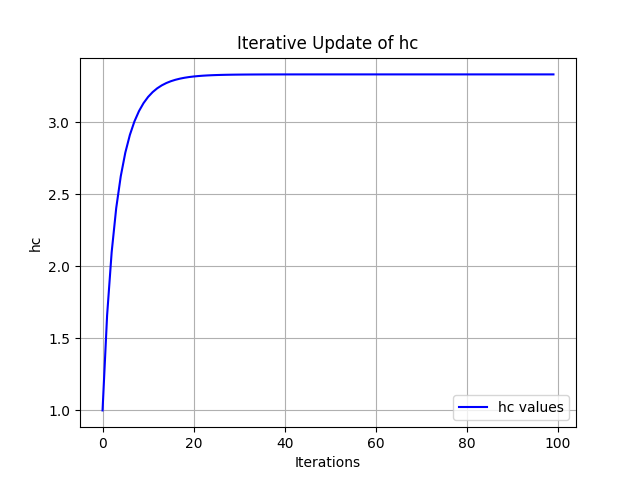
\includegraphics[width=\columnwidth]{figure/fig.png}
\end{figure}



 \end{document}
